\documentclass[a4paper,11pt]{article}
\usepackage[english]{babel}
\usepackage[T1]{fontenc}
\usepackage{fancyhdr}
\usepackage{graphicx}
\usepackage{a4wide}
\usepackage{numprint}
\usepackage{url}
\usepackage{cite}
\usepackage{multirow}
\usepackage{moreverb}
\usepackage{lastpage}
\usepackage{enumerate}
\pagestyle{fancy}

\author{Viktor Collin \\ <\url{vcollin@kth.se}> \\ 19880316-0277 \and Simon \"{O}sterman \\ <\url{simost@kth.se}> \\ 19880205-0156}
\title{\textbf{DH2323 Computer Graphics with Interaction \\ Lab 1 : Starfield}}

\fancyhead[L]{\textbf{DH2323 : Lab 1} }
\fancyhead[R]{Viktor Collin \& Simon \"{O}sterman : Page \thepage }
\fancyfoot{}{}

\begin{document}
\maketitle
\begin{center}
Total pages: \pageref{LastPage}
\end{center}
\thispagestyle{empty}

\clearpage
\setcounter{page}{1}
\section{Introduction}
This lab focuses on getting to know the basics of graphics programming such as the 
environments, libraries and simple algorithms to get started. After getting the environment running, the assignment is to write two programs; one in 2D and one in 3D. Below those two are explained in detail. 

\part{Interpolation}
\section{Problem statement}
The assignment here is basically to get SDL running and to linearly interpolate between pixels on the screen.

\section{Method}
We started by defining the colors on the four corners of the screen. Next, we interpolate vertically between the lower and upper left and right corners. When we have the borders, we interpolate horizontally to achieve the image required. 
\section{Result}
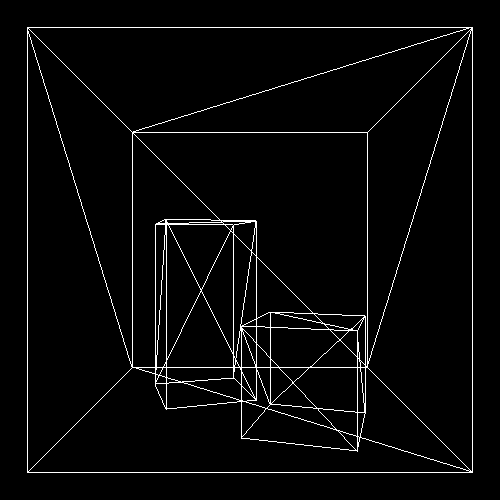
\includegraphics{screenshot1.pdf}

\clearpage
\part{Starfield}


\end{document}
